\newif\ifglobal

%%%%%%%%%%%%%%%%%%%%%%%
%%% Compile to view %%%
%%%%%%%%%%%%%%%%%%%%%%%

%%%%%%%%%%%%%%%%%%%%%%%%%%%%%%%%%%%%%%%%%%%%%%%%%%%
%%% Readme:                                     %%%
%%% https://www.overleaf.com/read/bwdjvfjksvjy/ %%%
%%%%%%%%%%%%%%%%%%%%%%%%%%%%%%%%%%%%%%%%%%%%%%%%%%%

% >>> M?: marks a module setting number or important notice

% >>> M4: Set {./relative-path} to external files for this module <<<
\def \modulefiles {./25-TWAI}
% To add an external file, use:
% (Replace '---' with actual filename)
% '\input{\modulefiles/tables/---.tex}' for tables
% '\includegraphics{\modulefiles/figures/---}' for figures
% '\subfile{\modulefiles/---}' for register files

% >>> M1: This module is in global project? <<<
% 'YES' - uncomment; 'NO' - comment out
\globaltrue

\ifglobal
    \documentclass[main\_\_EN.tex]{subfiles}

\else
    \documentclass[openany, 10pt]{book}

    % >>> M2: In ./00-shared/preamble-trm-module, also find
    %         settings for visibility of todo notes, watermark <<<
    \usepackage{preamble-trm-module}

    % >>> M3: Temporary labels in English,
    %         you can add your own labels there <<<
    \myexternaldocument{./00-shared/temp-labels-en}

\fi %\ifglobal


\setcounter{secnumdepth}{4}


% >>> M5: If this module needs any updates in
% './00-shared/preamble-trm-module.sty'
% (include additional package, etc.), contact your module PM
% or create the file './00-shared/changelog.tex' make the
% necessary updates yourself and document them in this file <<<

% Make text left-aligned and allow latex to break pages naturally, comment out for full justification
\raggedright
\raggedbottom


\begin{document}


% Sets language into which pre-defined bits of text are translated
\selectlanguage{english}
\setenglishformatting

% Do not delete this block
\ifglobal
% Add the following front matter if
% this module is outside of global project
\else
    \InputIfFileExists{readme}{}{}
    \listoftodos
    {\let\clearpage\relax \listofdonetodos}
    \tableofcontents
    %\listoftables
    %\listoffigures
\fi


%%%%%%%%%%%%%%%%%%%%%%%%%
%%% TRM Module Begins %%%
%%%%%%%%%%%%%%%%%%%%%%%%%

\hypertarget{twai}{}
\chapter{Two-Wire Automotive Interface (TWAI)}
\label{mod:twai}

\section{Overview}

The Two-wire Automotive Interface (TWAI$^\circledR$) is a multi-master, multi-cast communication protocol with error detection and signaling and inbuilt message priorities and arbitration.The TWAI protocol is suited for automotive and industrial applications (Please see \hyperref[subsec:protocol-description]{TWAI Protocol Description}).

ESP32 contains a TWAI controller that can be connected to a TWAI bus via an external transceiver. The TWAI controller contains numerous advanced features, and can be utilized in a wide range of use cases such as automotive products, industrial automation controls, building automation etc.

\section{Features}
ESP32 TWAI controller supports the following features:
\begin{itemize}
    \item compatible with ISO 11898-1 protocol (CAN Specification 2.0)
    \item Supports Standard Frame Format (11-bit ID) and Extended Frame Format (29-bit ID)
    \item Bit rates:
    \begin{itemize}
        \item from 25 Kbit/s to 1 Mbit/s in chip revision v0.0/v1.0/v1.1
        \item from 12.5 Kbit/s to 1 Mbit/s in chip revision v3.0/v3.1
    \end{itemize}
    \item Multiple modes of operation
    \begin{itemize}
        \item Normal
        \item Listen Only (no influence on bus)
        \item Self Test (transmissions do not require acknowledgment)
    \end{itemize}
    \item 64-byte Receive FIFO
    \item Special transmissions
    \begin{itemize}
        \item Single-shot transmissions (does not automatically re-transmit upon error)
        \item Self Reception (the TWAI controller transmits and receives messages simultaneously)
    \end{itemize}
    \item Acceptance Filter (supports single and dual filter modes)
    \item Error detection and handling
    \begin{itemize}
        \item Error counters
        \item Configurable Error Warning Limit
        \item Error Code Capture
        \item Arbitration Lost Capture
    \end{itemize}
\end{itemize}

\section{Functional Protocol}
\label{subsec:protocol-description}
\subsection{TWAI Properties}
The TWAI protocol connects two or more nodes in a bus network, and allows for nodes to exchange messages in a latency bounded manner. A TWAI bus will has a following properties.

{\bfseries Single Channel and Non-Return-to-Zero:} The bus consists of a single channel to carry bits, thus communication is half-duplex. Synchronization is also derived from this channel, thus extra channels (e.g., clock or enable) are not required. The bit stream of a TWAI message is encoded using the Non-Return-to-Zero (NRZ) method.

{\bfseries Bit Values:} The single channel can either be in a Dominant or Recessive state, representing a logical 0 and a logical 1 respectively. A node transmitting a Dominant state will always override a another node transmitting a Recessive state. The physical implementation on the bus is left to the application level to decide (e.g., differential wiring).

{\bfseries Bit-Stuffing:} Certain fields of TWAI messages are bit-stuffed. A Transmitter that transmits five consecutive bits of the same value should automatically insert a complementary bit. Likewise, a Receiver that receives five consecutive bits should treat the next bit as a stuff bit. Bit stuffing is applied to the following fields: SOF, Arbitration Field, Control Field, Data Field, and CRC Sequence (see Section \ref{subsubsec:twai-messages} for more details).

{\bfseries Multi-cast:} All nodes receive the same bits as they are connected to the same bus. Data is consistent across all nodes unless there is a bus error (See Section \ref{subsubsec:twai-errors}).

{\bfseries Multi-master:} Any node can initiate a transmission. If a transmission is already ongoing, a node will wait until the current transmission is over before beginning its own transmission.

{\bfseries Message-Priorities and Arbitration:} If two or more nodes simultaneously initiate a transmission, the TWAI protocol ensures that one node will win arbitration of the bus. The Arbitration Field of the message transmitted by each node is used to determine which node will win arbitration.

{\bfseries Error Detection and Signaling:} Each node will actively monitor the bus for errors, and signal the detection errors by transmitting an Error Frame.

{\bfseries Fault Confinement:} Each node will maintain a set of error counts that are incremented/decremented according to a set of rules. When the error counts surpass a certain threshold, a node will automatically eliminate itself from the network by switching itself off.

{\bfseries Configurable Bit Rate:} The bit rate for a single TWAI bus is configurable. However, all nodes within the same bus must operate at the same bit rate.

{\bfseries Transmitters and Receivers:} At any point in time, a TWAI node can either be a Transmitter or a Receiver.
\begin{itemize}
    \item A node originating a message is a Transmitter. The node remains a Transmitter until the bus is idle or until the node loses arbitration. Note that multiple nodes can be Transmitter if they have yet to lose arbitration.
    \item All nodes that are not Transmitters are Receivers.
\end{itemize}

\subsection{TWAI Messages}
\label{subsubsec:twai-messages}
TWAI nodes use messages to transmit data, and signal errors to other nodes. Messages are split into various frame types, and some frame types will have different frame formats.
The TWAI protocol has of the following frame types:

\begin{itemize}
    \item Data Frames
    \item Remote Frames
    \item Error Frames
    \item Overload Frames
    \item Interframe Space
\end{itemize}

The TWAI protocol has the following frame formats:
\begin{itemize}
    \item Standard Frame Format (SFF) that consists of a 11-bit identifier
    \item Extended Frame Format (EFF) that consists of a 29-bit identifier
\end{itemize}

\subsubsection{Data Frames and Remote Frames}
Data Frames are used by nodes to send data to other nodes, and can have a payload of 0 to 8 data bytes. Remote Frames are used to nodes to request a Data Frame with the same Identifier from another node, thus does not contain any data bytes. However, Data Frames and Remote Frames share many common fields. Figure \ref{Figure:Bit Fields} illustrates the fields and sub fields of the different frames and formats.

\begin{figure}[ht!]
    \centering
    \fbox{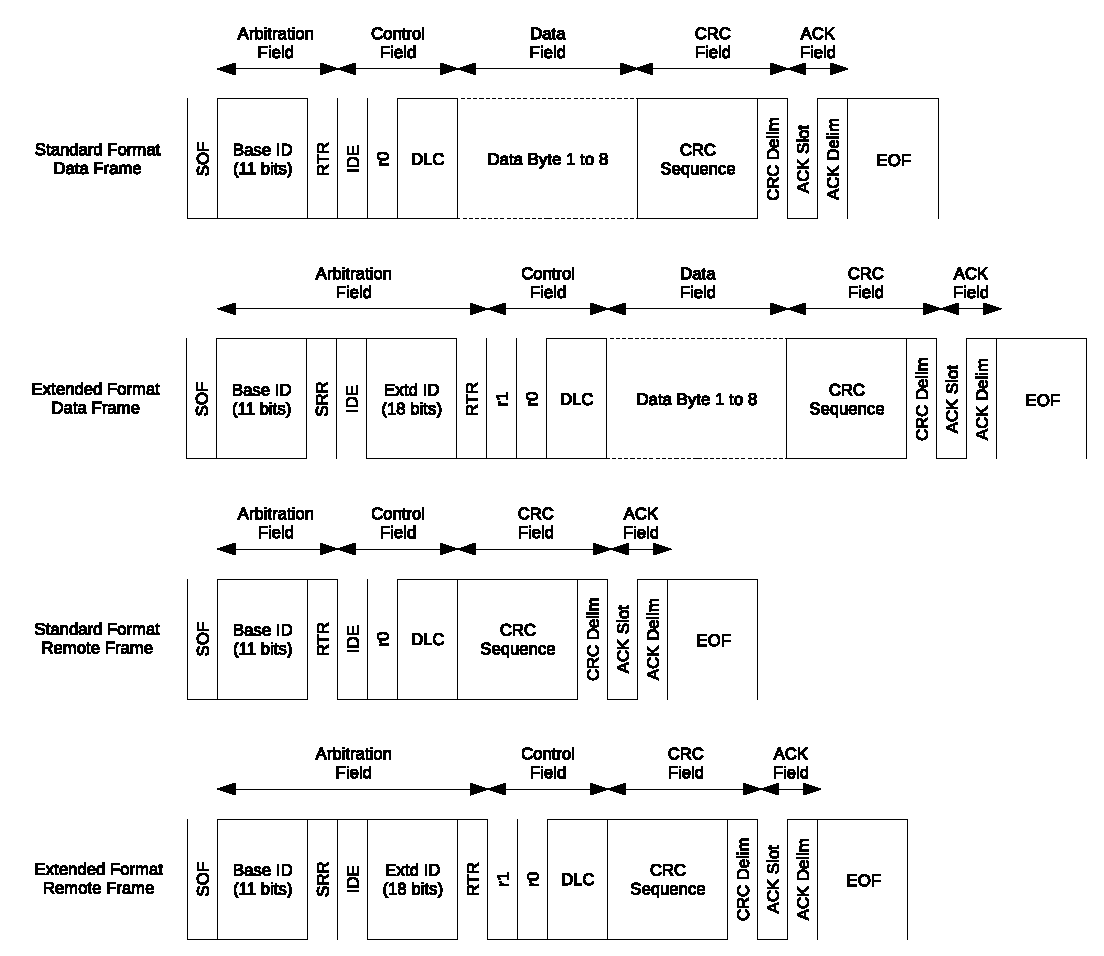
\includegraphics[width=0.8\textwidth]{./25-TWAI/figures/Bit_Fields_en.eps}}
    \caption{The bit fields of Data Frames and Remote Frames}
    \label{Figure:Bit Fields}
\end{figure}


{\bfseries Arbitration Field}\\

When two or more nodes transmits a Data or Remote Frame simultaneously, the Arbitration Field is used to determine which node will win arbitration of the bus. During the Arbitration Field, if a node transmits a Recessive bit but observes a Dominant bit, this indicates that another node has overridden its Recessive bit. Therefore, the node transmitting the Recessive bit has lost arbitration of the bus and should immediately become a Receiver.

The Arbitration Field primarily consists of the Frame Identifier that is transmitted most significant bit first. Given that a Dominant bit represents a logical 0, and a Recessive bit represents a logical 1:

\begin{itemize}
    \item A frame with the smallest ID value will always win arbitration.
    \item Given the same ID and format, Data Frames will always prevail over RTR Frames.
    \item Given the same first 11 bits of ID, a Standard Format Data Frame will prevail over an Extended Format Data Frame due to the SRR being recessive.
\end{itemize}


{\bfseries Control Field}\\

The control field primarily consists of the DLC (Data Length Code) which indicates the number of payload data bytes for a Data Frame, or the number of requested data bytes for a Remote Frame. The DLC is transmitted most significant bit first.

{\bfseries Data Field}\\

The Data Field contains the actual payload data bytes of a Data Frame. Remote Frames do not contain a Data Field.

{\bfseries CRC Field}\\

The CRC Field primarily consists of a a CRC Sequence. The CRC Sequence is a 15-bit cyclic redundancy code calculated form the de-stuffed contents (everything from the SOF to the end of the Data Field) of a Data or Remote Frame.

{\bfseries ACK Field}\\
The ACK Field primarily consists of an ACK Slot and an ACK Delim. The ACK Field is mainly intended for the receiver to send a message to a transmitter, indicating it has received an effective message.

\begin{longtable}[c]{|p{3.5cm}|p{12cm}|}

  \caption{Data Frames and Remote Frames in SFF and EFF}
  \label{table:Data Frames and Remote Frames}
  \\\hline
  \rowcolor{lightgray}
  {Data/Remote Frames} & {Description}
  \\\hline
  \endfirsthead

  \hline
  \rowcolor{lightgray}
   {Data/Remote Frames} & {Description}
   \\\hline
  \endhead
  \endfoot
  \hline
  \endlastfoot

    SOF & The SOF (Start of Frame) is a single Dominant bit used to synchronize nodes on the bus.
          \\\hline
    Base ID & The Base ID (ID.28 to ID.18) is the 11-bit Identifier for SFF, or the first 11-bits of the 29-bit Identifier for EFF.                     \\\hline
    RTR & The RTR (Remote Transmission Request) bit indicates whether the message is a Data Frame (Dominant) or a Remote Frame (Recessive). This means that a Remote Frame will always lose arbitration to a Data Frame given they have the same ID.                                               \\\hline
    SRR & The SRR (Substitute Remote Request) bit is transmitted in EFF to substitute for the RTR bit at the same position in SFF.                       \\\hline
    IDE & The IDE (Identifier Extension) bit indicates whether the message is SFF (Dominant) or EFF (Recessive). This means that a SFF frame will always win arbitration over an EFF frame given they have the same Base ID.                       \\\hline
    Extd ID & The Extended ID (ID.17 to ID.0) is the remaining 18-bits of the 29-bit identifier for EFF.                                                \\\hline
    r1 & The r1 (reserved bit 1) is always Dominant.
             \\\hline
    r0 & The r0 (reserved bit 0) is always Dominant.
             \\\hline
    DLC & The DLC (Data Length Code) is 4-bits and should have a value from 0 to 8. Data Frames use the DLC to indicate the number data bytes in the Data Frame. Remote Frames used the DLC to indicate the number of data bytes to request from another node.
             \\\hline
    Data Bytes & The data payload of Data Frames. The number of bytes should match the value of DLC. Data byte 0 is transmitted first, and each data byte is transmitted most significant bit first.
             \\\hline
    CRC Sequence & The CRC sequence is a 15-bit cyclic redundancy code.
             \\\hline
    CRC Delim & The CRC Delim (CRC Delimiter) is a single Recessive bit that follows the CRC sequence.
              \\\hline
    ACK Slot & The ACK Slot (Acknowledgment Slot) that intended for Receiver nodes to indicate that the Data or Remote Frame was received without issue. The Transmitter node will send a Recessive bit in the ACK Slot and Receiver nodes should override the ACK Slot with a Dominant bit if the frame was received without errors.
              \\\hline
    ACK Delim & The ACK Delim (Acknowledgment Delimiter) is a single Recessive bit.
              \\\hline
    EOF & The EOF (End of Frame) marks the end of a Data or Remote Frame, and consists of seven Recessive bits.
              \\\hline

\end{longtable}

\subsubsection{Error and Overload Frames}

{\bfseries Error Frames}

Error Frames are transmitted when a node detects a Bus Error. Error Frames notably consist of an Error Flag which is made up of 6 consecutive bits of the same value, thus violating the bit-stuffing rule. Therefore, when a particular node detects a Bus Error and transmits an Error Frame, all other nodes will then detect a Stuff Error and transmit their own Error Frames in response. This has the effect of propagating the detection of a Bus Error across all nodes on the bus.
When a node detects a Bus Error, it will transmit an Error Frame starting on the next bit. However, if the type of Bus Error was a CRC Error, then the Error Frame will start at the bit following the ACK Delim (see Section \ref{subsubsec:twai-errors}). The following Figure \ref{Figure:Fields of an Error Frame} shows the various fields of an Error Frame:

\begin{figure}[ht]
    \centering
    \fbox{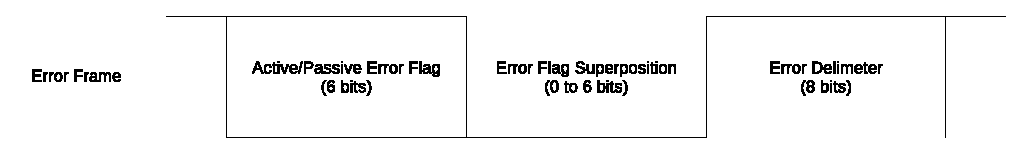
\includegraphics[width=0.85\textwidth]{./25-TWAI/figures/Fields_of_an_Error_Frame_en.eps}}
    \caption{Various Fields of an Error Frame}
    \label{Figure:Fields of an Error Frame}
\end{figure}

\begin{longtable}[c]{|p{4cm}|p{11cm}|}

  \caption{Error Frame}
  \label{table:Error_Frame}
  \\\hline
  \rowcolor{lightgray}
  {Error Frame} & {Description}
  \\\hline
  \endfirsthead

  \hline
  \rowcolor{lightgray}
   {Error Frame} & {Description}
   \\\hline
  \endhead
  \endfoot
  \hline
  \endlastfoot

    Error Flag & The Error Flag has two forms, the Active Error Flag consisting of 6 Dominant bits and the Passive Error Flag consisting of 6 Recessive bits (unless overridden by Dominant bits of other nodes). Active Error Flags are sent by Error Active nodes, whilst Passive Error Flags are sent by Error Passive nodes.
          \\\hline
    Error Flag Superposition & The Error Flag Superposition field meant to allow for other nodes on the bus to transmit their respective Active Error Flags. The superposition field can range from 0 to 6 bits, and ends when the first Recessive bit is detected (i.e., the first it of the Delimiter).                               \\\hline
    Error Delimiter & The Delimiter field marks the end of the Error/Overload Frame, and consists of 8 Recessive bits.                                                          \\\hline

\end{longtable}

{\bfseries Overload Frames}\\

An Overload Frame has the same bit fields as an Error Frame containing an Active Error Flag. The key difference is in the conditions that can trigger the transmission of an Overload Frame. Figure \ref{Figure:Bit Fields of an Overload Frame} below shows the bit fields of an Overload Frame.
\begin{figure}[H]
    \centering
    \fbox{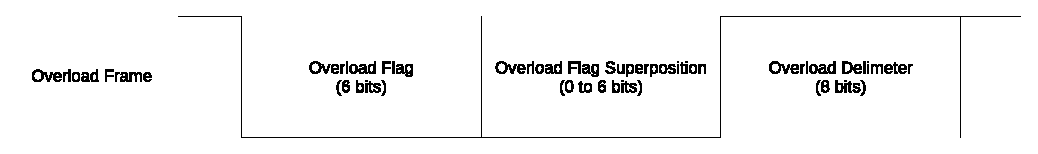
\includegraphics[width=0.85\textwidth]{./25-TWAI/figures/Overload_frames_en.eps}}
    \caption{The Bit Fields of an Overload Frame}
    \label{Figure:Bit Fields of an Overload Frame}
\end{figure}

\begin{longtable}[c]{|p{4cm}|p{11cm}|}

  \caption{Overload Frame}
  \label{table:Overload_Frames}
  \\\hline
  \rowcolor{lightgray}
  Overload Frame & Description
  \\\hline
  \endfirsthead

  \hline
  \rowcolor{lightgray}
   Overload Frame & Description
   \\\hline
  \endhead
  \endfoot
  \hline
  \endlastfoot

    Overload Flag & Consists of 6 Dominant bits. Same as an Active Error Flag.
          \\\hline
    Overload Flag Superposition & Allows for the superposition of Overload Flags from other nodes, similar to an Error Flag Superposition.
           \\\hline
    Overload Delimiter & Consists of 8 Recessive. Same as an Error Delimiter.                                           \\\hline

\end{longtable}

Overload Frames will be transmitted under the following conditions:
\begin{enumerate}
    \item The internal conditions of a Receiver requires a delay of the next Data or Remote Frame.
    \item Detection of a Dominant bit at the first and second bit of Intermission.
    \item If a Dominant bit is detected at the eighth (last) bit of an Error Delimiter. Note that in this case, TEC and REC will not be incremented (See Section \ref{subsubsec:twai-errors}).
\end{enumerate}
Transmitting an overload frame due to one of the conditions must also satisfy the following rules:
\begin{itemize}
    \item Transmitting an Overload Frame due to condition 1 must only be started at the first bit of Intermission.
    \item Transmitting an Overload Frame due to condition 2 and 3 must start one bit after the detecting the Dominant bit of the condition.
    \item A maximum of two Overload frames may be generated in order to delay the next Data or Remote Frame.
\end{itemize}


\subsubsection{Interframe Space}

The Interframe Space acts as a separator between frames. Data Frames and Remote Frames must be separated from preceding frames by an Interframe Space, regardless of the preceding frame’s type (Data Frame, Remote Frame, Error Frame, Overload Frame). However, Error Frames and Overload Frames do not need to be separated from preceding frames.

Figure \ref{Figure:The Fields within an Interframe Space} shows the fields within an Interframe Space:

\begin{figure}[ht]
    \centering
    \fbox{
\includegraphics[width=0.85\textwidth]{./25-TWAI/figures/Fields_within_an_Interframe_Space_en.eps}}
    \caption{The Fields within an Interframe Space}
    \label{Figure:The Fields within an Interframe Space}
\end{figure}

\begin{longtable}[c]{|p{4cm}|p{11cm}|}
  \caption{Interframe Space}
  \label{table:Interframe_space}
  \\\hline
  \rowcolor{lightgray}
  Interframe Space & Description
  \\\hline
  \endfirsthead

  \hline
  \rowcolor{lightgray}
   Interframe Space & Description
   \\\hline
  \endhead
  \endfoot
  \hline
  \endlastfoot

    Intermission & The Intermission consists of 3 Recessive bits.
           \\\hline
    Suspend Transmission & An Error Passive node that has just transmitted a message must include a Suspend Transmission field. This field consists of 8 Recessive bits. Error Active nodes should not include this field.
            \\\hline
    Bus Idle & The Bus Idle field is of arbitrary length. Bus Idle ends when an SOF is transmitted. If a node has a pending transmission, the SOF should be transmitted at the first bit following Intermission.
             \\\hline
    \end{longtable}

\subsection{TWAI Errors}
\label{subsubsec:twai-errors}
\subsubsection{Error Types}

Bus Errors in TWAI are categorized into one of the following types:

{\bfseries Bit Error}\\
A Bit Error occurs when a node transmits a bit value (i.e., Dominant or Recessive) but the opposite bit is detected (e.g., a Dominant bit is transmitted but a Recessive is detected). However, if the transmitted bit is Recessive and is located in the Arbitration Field or ACK Slot or Passive Error Flag, then detecting a Dominant bit will not be considered a Bit Error.


{\bfseries Stuff Error}\\
A stuff error is detected when 6 consecutive bits of the same value are detected (thus violating the bit-stuffing encoding).

{\bfseries CRC Error}\\
A Receiver of a Data or Remote Frame will calculate a CRC based on the bits it has received. A CRC error occurs when the CRC calculated by the Receiver does not match the CRC sequence in the received Data or Remote Frame.

{\bfseries Form Error}\\
A Form Error is detected when a fixed-form bit field of a message contains an illegal bit. For example, the r1 and r0 fields must be Dominant.

{\bfseries Acknowledgement Error}\\
An Acknowledgment Error occurs when a Transmitter does not detect a Dominant bit at the ACK Slot.

\subsubsection{Error States}
TWAI nodes implement fault confinement by each maintaining two error counters, where the counter values determine the error state. The two error counters are known as the Transmit Error Counter (TEC) and Receive Error Counter (REC). TWAI has the following error states.

{\bfseries Error Active}\\
An Error Active node is able to participate in bus communication and transmit an Active Error Flag when it detects an error.

{\bfseries Error Passive}\\
An Error Passive node is able to participate in bus communication, but can only transmit an Passive Error Flag when it detects an error. Error Passive nodes that have transmitted a Data or Remote Frame must also include the Suspend Transmission field in the subsequent Interframe Space.

{\bfseries Bus Off}\\
A Bus Off node is not permitted to influence the bus in any way (i.e., is not allowed to transmit anything).

\subsubsection{Error Counters}

The TEC and REC are incremented/decremented according to the following rules. {\bfseries Note that more than one rule can apply for a given message transfer.}

\begin{enumerate}
    \item When a Receiver detects an error, the REC will be increased by 1, except when the detected error was a Bit Error during the transmission of an Active Error Flag or an Overload Flag.
    \item When a Receiver detects a Dominant bit as the first bit after sending an Error Flag, the REC will be increased by 8.
    \item When a Transmitter sends an Error Flag the TEC is increased by 8. However, the following scenarios are exempt form this rule:
    \begin{itemize}
        \item If a Transmitter is Error Passive that detects an Acknowledgment Error due to not detecting a Dominant bit in the ACK slot, it should send a Passive Error Flag. If no Dominant bit is detected in that Passive Error Flag, the TEC should not be increased.
        \item A Transmitter transmits an Error Flag due to a Stuff Error during Arbitration. If the offending bit should have been Recessive but was monitored as Dominant, then the TEC should not be increased.
    \end{itemize}
    \item If a Transmitter detects a Bit Error whilst sending an Active Error Flag or Overload Flag, the REC is increased by 8.
    \item If a Receiver detects a Bit Error while sending an Active Error Flag or Overload Flag, the REC is increased by 8.
    \item Any node tolerates up to 7 consecutive Dominant bits after sending an Active/Passive Error Flag, or Overload Flag. After detecting the 14th consecutive Dominant bit (when sending an Active Error Flag or Overload Flag), or the 8th consecutive Dominant bit following a Passive Error Flag, a Transmitter will increase its TEC by 8 and a Receiver will increase its REC by 8. Each additional eight consecutive Dominant bits will also increase the TEC (for Transmitters) or REC (for Receivers) by 8 as well.
    \item When a Transmitter successfully transmits a message (getting ACK and no errors until the EOF is complete), the TEC is decremented by 1, unless the TEC is already at 0.
    \item When a Receiver successfully receives a message (no errors before ACK Slot, and successful sending of ACK), the REC is decremented.
    \begin{itemize}
        \item If the REC was between 1 and 127, the REC is decremented by 1.
        \item If the REC was greater than 127, the REC is set to 127.
        \item If the REC was 0, the REC remains 0.
    \end{itemize}
    \item A node becomes Error Passive when its TEC and/or REC is greater than or equal to 128. The error condition that causes a node to become Error Passive will cause the node to send an Active Error Flag. Note that once the REC has reached to 128, any further increases to its value are irrelevant until the REC returns to a value less than 128.
    \item A node becomes Bus Off when its TEC is greater than or equal to 256.
    \item An Error Passive node becomes Error Active when both the TEC and REC are less than or equal to 127.
    \item A Bus Off node can become Error Active (with both its TEC and REC reset to 0) after it monitors 128 occurrences of 11 consecutive Recessive bits on the bus.
\end{enumerate}

\subsection{TWAI Bit Timing}
\subsubsection{Nominal Bit}

The TWAI protocol allows a TWAI bus to operate at a particular bit rate. However, all nodes within a TWAI bus must operate at the same bit rate.

\begin{itemize}
    \item The \textbf{Nominal Bit Rate} is defined as number of bits transmitted per second from an ideal Transmitter and without any synchronization.
    \item The \textbf{Nominal Bit Time} is defined as \textbf{1/Nominal Bit Rate}.
\end{itemize}

A single Nominal Bit Time is divided into multiple segments, and each segment is made up of multiple Time Quanta. A {\bfseries Time Quantum} is a fixed unit of time, and is implemented as some form of prescaled clock signal in each node. Figure \ref{Figure:TWAI_BIT_TIMING} illustrates the segments within a single Nominal Bit Time.

TWAI Controllers will operate in time steps of one Time Quanta where the state of the TWAI bus is analyzed at every Time Quanta. If two consecutive Time Quantas have different bus states (i.e., Recessive to Dominant or vice versa), this will be considered an edge. When the bus is analyzed at the intersection of PBS1 and PBS2, this is considered the Sample Point and the sampled bus value is considered the value of that bit.

\begin{figure}[ht]
    \centering
    \fbox{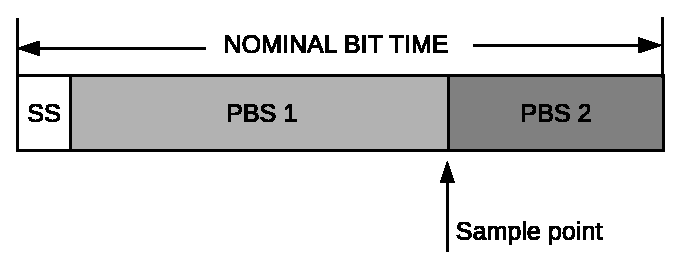
\includegraphics[width=0.6\textwidth]{./25-TWAI/figures/TWAI_BIT_TIMING_20190625_en.eps}}
    \caption{Layout of a Bit}
    \label{Figure:TWAI_BIT_TIMING}
\end{figure}

\begin{longtable}[c]{|p{2.5cm}|p{13cm}|}

  \caption{Segments of a Nominal Bit Time}
  \label{table:Segments of a Nominal Bit Time}
  \\\hline
  \rowcolor{lightgray}
  {Segment} & {Description}
  \\\hline
  \endfirsthead

  \hline
  \rowcolor{lightgray}
   {Segment} & {Description}
   \\\hline
  \endhead
  \endfoot
  \hline
  \endlastfoot

    SS & The SS (Synchronization Segment) is 1 Time Quantum long. If all nodes are perfectly synchronized, the edge of a bit will lie in the SS.
            \\\hline
    PBS1 & PBS1 (Phase Buffer Segment 1) can be 1 to 16 Time Quanta long. PBS1 is meant to compensate for the physical delay times within the network. PBS1 can also be lengthened for synchronization purposes.
            \\\hline
    PBS2 & PBS2 (Phase Buffer Segment 2) can be 1 to 8 Time Quanta long. PBS2 is meant to compensate for the information processing time of nodes. PBS2 can also be shortened for synchronization purposes.
            \\\hline

\end{longtable}

\subsubsection{Hard Synchronization and Resynchronization}

Due to clock skew and jitter, the bit timing of nodes on the same bus may become out of phase. Therefore, a bit edge may come before or after the SS. To ensure that the internal bit timing clocks of each node are kept in phase, TWAI has various methods of synchronization. The \textbf{Phase Error “e”} is measured in the number of Time Quanta and relative to the SS.

\begin{itemize}
    \item A positive Phase Error (e > 0) is when the edge lies after the SS and before the Sample Point (i.e., the edge is late).
    \item A negative Phase Error (e < 0) is when the edge lies after the Sample Point of the previous bit and before SS (i.e., the edge is early).
\end{itemize}

To correct for Phase Errors, there are two forms of synchronization, known as \textbf{Hard Synchronization} and \textbf{Resynchronization}. \textbf{Hard Synchronization} and \textbf{Resynchronization} obey the following rules.

\begin{itemize}
    \item Only one synchronization may occur in a single bit time.
    \item Synchronizations only occurs on Recessive to Dominant edges.
\end{itemize}

{\bfseries Hard Synchronization}\\
Hard Synchronization occurs on the Recessive to Dominant edges during Bus Idle (i.e., the SOF bit). All nodes will restart their internal bit timings such that the Recessive to Dominant edge lies within the SS of the restarted bit timing.

{\bfseries Resynchronization}\\
Resynchronization occurs on Recessive to Dominant edges not during Bus Idle. If the edge has a positive Phase Error (e > 0), PBS1 is lengthened by a certain number of Time Quanta. If the edge has a negative Phase Error (e < 0), PBS2 will be shortened by a certain number of Time Quanta.

The number of Time Quanta to lengthen or shorten depends on the magnitude of the Phase Error, and is also limited by the Synchronization Jump Width (SJW) value which is a programmable.

\begin{itemize}
    \item When the magnitude of the Phase Error is less than or equal to the SJW, PBS1/PBS2 are lengthened/shortened by \textbf{e} number of Time Quanta. This has a same effect as Hard Synchronization.
    \item When the magnitude of the Phase Error is greater to the SJW, PBS1/PBS2 are lengthened/shortened by the SJW number of Time Quanta. This means it may take multiple bits of synchronization before the Phase Error is entirely corrected.
\end{itemize}

\section{Architectural Overview}
\begin{figure}[ht]
    \centering
    \fbox{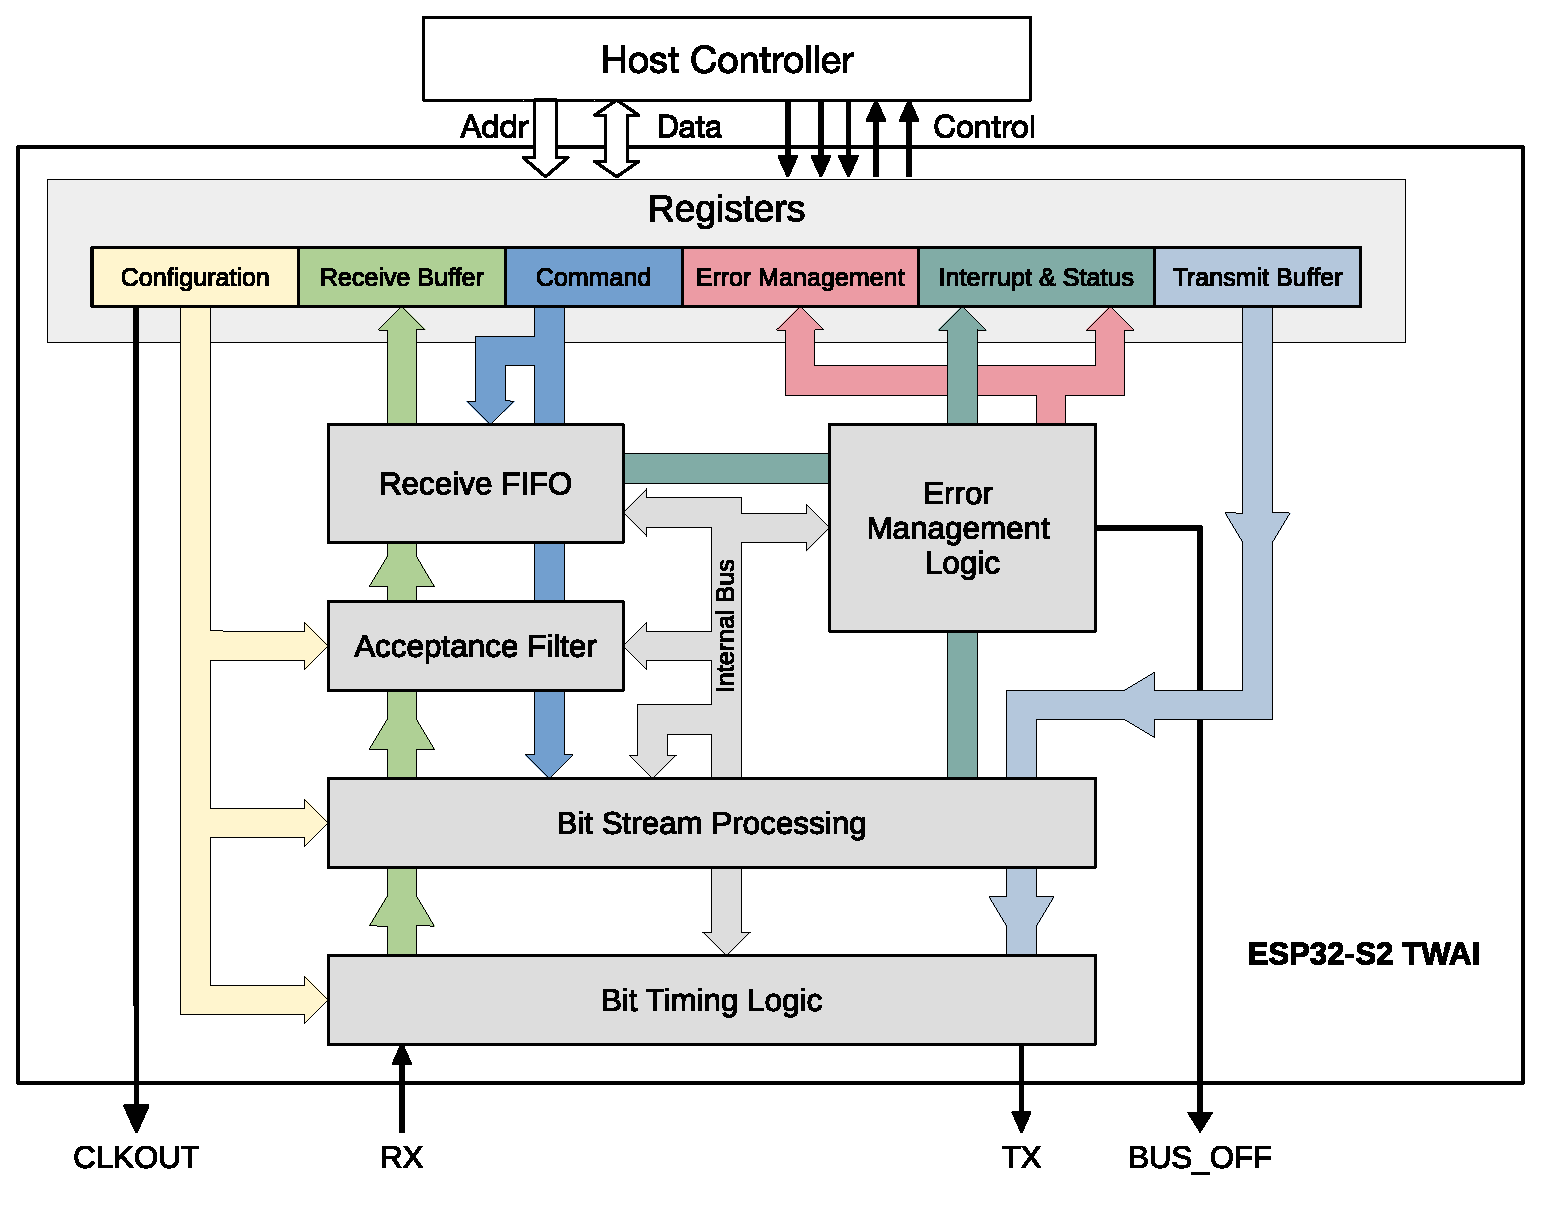
\includegraphics[width=0.8\textwidth]{./25-TWAI/figures/TWAI_Overview_Diagram_20190628.eps}}
    \caption{TWAI Overview Diagram}
    \label{Figure:TWAI Overview Diagram}
\end{figure}

The ESP32 contains a TWAI Controller. Figure \ref{Figure:TWAI Overview Diagram} shows the major functional blocks of the TWAI Controller.

\subsection{Registers Block}
The ESP32 CPU accesses peripherals as 32-bit aligned words. However, the majority of registers in the TWAI controller only contain useful data at the least significant byte (bits [7:0]). Therefore, in these registers, bits [31:8] are ignored on writes, and return 0 on reads.

{\bfseries Configuration Registers}\\
The configuration registers store various configuration options for the TWAI controller such as bit rates, operating mode, Acceptance Filter etc. Configuration registers can only be modified whilst the TWAI controller is in Reset Mode (See Section \ref{subsubsec:modes}).

{\bfseries Command Register}\\
The command register is used by the CPU to drive the TWAI controller to initiate certain actions such as transmitting a message or clearing the Receive Buffer. The command register can only be modified when the TWAI controller is in Operation Mode (see section \ref{subsubsec:modes}).


{\bfseries Interrupt \verb+&+ Status Registers}\\
The interrupt register indicates what events have occurred in the TWAI controller (each event is represented by a separate bit). The status register indicates the current status of the TWAI controller.

{\bfseries Error Management Registers}\\

The error management registers include error counters and capture registers. The error counter registers
represent TEC and REC values. The capture registers will record information about instances where TWAI controller detects a bus error, or when it loses arbitration.

{\bfseries Transmit Buffer Registers}\\
The transmit buffer is a 13-byte buffer used to store a TWAI message to be transmitted.

{\bfseries Receive Buffer Registers}\\
The Receive Buffer is a 13-byte buffer which stores a single message. The Receive Buffer acts as a window into Receive FIFO mapping to the first received message in the Receive FIFO to the Receive Buffer.

Note that the Transmit Buffer registers, Receive Buffer registers, and the Acceptance Filter registers share the same address range (offset 0x0040 to 0x0070). Their access is governed by the following rules:

\begin{itemize}
    \item When the TWAI controller is in Reset Mode, the address range maps to the Acceptance Filter registers.
    \item When the TWAI controller is in Operation Mode:
    \begin{itemize}
        \item All reads to the address range maps to the Receive Buffer registers.
        \item All writes to the address range maps to the Transmit Buffer registers.
    \end{itemize}
\end{itemize}

\subsection{Bit Stream Processor}
The Bit Stream Processing (BSP) module is responsible for framing data from the Transmit Buffer (e.g. bit stuffing and additional CRC fields) and generating a bit stream for the Bit Timing Logic (BTL) module. At the same time, the BSP module is also responsible for processing the received bit stream (e.g., de-stuffing and verifying CRC) from the BTL module and placing the message into the Receive FIFO. The BSP will also detect errors on the TWAI bus and report them to the Error Management Logic (EML).


\subsection{Error Management Logic}
The Error Management Logic (EML) module is responsible for updating the TEC and REC, recording error information like error types and positions, and updating the error state of the TWAI Controller such that the BSP module generates the correct Error Flags. Furthermore, this module also records the bit position when the TWAI controller loses arbitration.

\subsection{Bit Timing Logic}
The Bit Timing Logic (BTL) module is responsible for transmitting and receiving messages at the configured bit rate. The BTL module also handles synchronization of out of phase bits such that communication remains stable. A single bit time consists of multiple programmable segments that allows users to set the length of each segment to account for factors such as propagation delay and controller processing time etc.

\subsection{Acceptance Filter}
The Acceptance Filter is a programmable message filtering unit that allows the TWAI controller to accept or reject a received message based on the message’s ID field. Only accepted messages will be stored in the Receive FIFO. The Acceptance Filter’s registers can be programmed to specify a single filter, or specify two separate filters (dual filter mode).

\subsection{Receive FIFO}
The Receive FIFO is a 64-byte buffer (internal to the TWAI controller) that stores received messages accepted by the Acceptance Filter. Messages in the Receive FIFO can vary in size (between 3 to 13-bytes). When the Receive FIFO is full (or does not have enough space to store the next received message in its entirety), the Overrun Interrupt will be triggered, and any subsequent received messages will be lost until adequate space is cleared in the Receive FIFO. The first message in the Receive FIFO will be mapped to the 13-byte Receive Buffer until that message is cleared (using the Release Receive Buffer command bit). After clearing, the Receive Buffer will map to the next message in the Receive FIFO, and the space occupied by the previous message in the Receive FIFO can be used to receive new messages.

\section{Functional Description}

\subsection{Modes}
\label{subsubsec:modes}
The ESP32 TWAI controller has two working modes: Reset Mode and Operation Mode. Reset Mode and Operation Mode are entered by setting the \hyperref[fielddesc:TWAIRESETMODE]{TWAI\_RESET\_MODE} bit to 1 or 0 respectively.

\subsubsection{Reset Mode}
Entering Reset Mode is required in order to modify the various configuration registers of the TWAI controller. When entering Reset Mode, the TWAI controller is essentially disconnected from the TWAI bus. When in Reset Mode, the TWAI controller will not be able to transmit any messages (including error signaling). Any transmission in progress is immediately terminated. Likewise, the TWAI controller will also not be able to receive any messages.

\subsubsection{Operation Mode}
Entering Operation Mode essentially connects the TWAI controller to the TWAI bus, and write protects the TWAI controller’s configuration registers ensuring the configuration stays consistent during operation. When in Operation Mode, the TWAI controller can transmit and receive messages (including error signaling) depending on which operating sub-mode the TWAI controller was configured with. The TWAI controller supports the following operating sub-modes:

\begin{itemize}
    \item {\bfseries Normal Mode:} The TWAI controller can transmit and receive messages including error signaling (such as Error and Overload Frames).
    \item {\bfseries Self Test Mode:} Like Normal Mode, but the TWAI controller will consider the transmission of a Data or RTR Frame successful even if it was not acknowledged. This is commonly used when self testing the TWAI controller.
    \item {\bfseries Listen Only Mode:} The TWAI controller will be able to receive messages, but will remain completely passive on the TWAI bus. Thus, the TWAI controller will not be able to transmit any messages, acknowledgments, or error signals. The error counters will remain frozen. This mode is useful for TWAI bus monitors.
\end{itemize}

Note that when exiting Reset Mode (i.e., entering Operation Mode), the TWAI controller must wait for 11 consecutive Recessive bits to occur before being able to fully connect the TWAI bus (i.e., be able to transmit or receive).

\subsection{Bit Timing}
The operating bit rate of the TWAI controller must be configured whilst the TWAI controller is in Reset Mode. The bit rate configuration is located in \hyperref[regdesc:TWAIBUSTIMING0REG]{TWAI\_BUS\_TIMING\_0\_REG} and \hyperref[regdesc:TWAIBUSTIMING1REG]{TWAI\_BUS\_TIMING\_1\_REG}, and the two registers contain the following fields:

The following Table \ref{table:Bit_timing_0} illustrates the bit fields of \hyperref[regdesc:TWAIBUSTIMING0REG]{TWAI\_BUS\_TIMING\_0\_REG}.

\begin{longtable}[c]{|p{1.4cm}|p{1.4cm}|p{1.4cm}|p{1.4cm}|p{1.4cm}|p{1.4cm}|p{1.4cm}|p{1.4cm}|p{1.4cm}|}
\caption{Bit Information of \hyperref[regdesc:TWAICLOCKDIVIDERREG]{TWAI\_CLOCK\_DIVIDER\_REG}; TWAI Address 0x18}
\label{table:Bit_timing_0}\\\hline
\rowcolor{lightgray}
   Bit 31-8 & Bit 7 & Bit 6 & Bit 5 & Bit 4 & Bit 3 & Bit 2 & Bit 1 & Bit 0\\\hline
  Reserved & SJW.1 & SJW.0 & BRP.5 & BRP.4 & BRP.3 & BRP.2 & BRP.1 & BRP.0\\\hline
\end{longtable}
\vspace{-1.5em}
{\bfseries Notes:}\\
\begin{itemize}
    \item SJW: Synchronization Jump Width (SJW) is configured in SJW.0 and SJW.1 where SJW = (2 x SJW.1 + SJW.0 + 1).
    \item BRP: The TWAI Time Quanta clock is derived from a prescaled version of the APB clock that is usually 80 MHz. The Baud Rate Prescaler (BRP) field is used to define the prescaler according to the equation below, where t$_{Tq}$ is the Time Quanta clock period and t$_{CLK}$ is APB clock period :\\

t$_{Tq}$ = 2 × t$_{CLK}$ × (2$^{5}$ × BRP.5 + 2$^{4}$ × BRP.4 + 2$^{3}$ × BRP.3 + 2$^2$ × BRP.2 + 2$^1$ × BRP.1 + 2$^0$ × BRP.0 + 1)
\end{itemize}

The following Table \ref{table:Bit_timing_1} illustrates the bit fields of \hyperref[regdesc:TWAIBUSTIMING1REG]{TWAI\_BUS\_TIMING\_1\_REG}.

\begin{longtable}[c]{|p{1.4cm}|p{1.4cm}|p{1.4cm}|p{1.4cm}|p{1.4cm}|p{1.4cm}|p{1.4cm}|p{1.4cm}|p{1.4cm}|}
    \caption{Bit Information of \hyperref[regdesc:TWAIBUSTIMING1REG]{TWAI\_BUS\_TIMING\_1\_REG}; TWAI Address 0x1c}
    \label{table:Bit_timing_1}\\
    \hline
       \rowcolor{lightgray}
   Bit 31-8 & Bit 7 & Bit 6 & Bit 5 & Bit 4 & Bit 3 & Bit 2 & Bit 1 & Bit 0\\\hline
   Reserved & SAM & PBS2.2 & PBS2.1 & PBS2.0 & PBS1.3 &PBS1.2 & PBS1.1 & PBS1.0\\
    \hline
\end{longtable}
\vspace{-1.5em}
{\bfseries Notes:}\\
\begin{itemize}
    \item PBS1: The number of Time Quanta in Phase Buffer Segment 1 is defined according to the following equation: (8 x PBS1.3 + 4 x PBS1.2 + 2 x PBS1.1 + PBS1.0 + 1).
    \item PBS2: The number of Time Quanta in Phase Buffer Segment 2 is defined according to the following equation: (4 x PBS2.2 + 2 x PBS2.1 + PBS2.0 + 1).
    \item SAM: Enables triple sampling if set to 1. This is useful for low/medium speed buses where filtering spikes on the bus line is beneficial.
\end{itemize}

\subsection{Interrupt Management}
\label{subsubsec:interrupt-management}
The ESP32 TWAI controller provides seven interrupts, each represented by a single bit in the \hyperref[regdesc:TWAIINTRAWREG]{TWAI\_INT\_RAW\_REG}. For a particular interrupt to be triggered (i.e., its bit in \hyperref[regdesc:TWAIINTRAWREG]{TWAI\_INT\_RAW\_REG} set to 1), the interrupt’s corresponding enable bit in \hyperref[regdesc:TWAIINT ENAREG]{TWAI\_INT ENA\_REG} must be set.

The TWAI controller provides the seven following interrupts:

\begin{itemize}
    \item Receive Interrupt
    \item Transmit Interrupt
    \item Error Warning Interrupt
    \item Data Overrun Interrupt
    \item Error Passive Interrupt
    \item Arbitration Lost Interrupt
    \item Bus Error Interrupt
\end{itemize}

The TWAI controller’s interrupt signal to the interrupt matrix will be asserted whenever one or more interrupt bits are set in the \hyperref[regdesc:TWAIINTRAWREG]{TWAI\_INT\_RAW\_REG}, and deasserted when all bits in \hyperref[regdesc:TWAIINTRAWREG]{TWAI\_INT\_RAW\_REG} are cleared. The majority of interrupt bits in \hyperref[regdesc:TWAIINTRAWREG]{TWAI\_INT\_RAW\_REG} are automatically cleared when the register is read. However, the Receive Interrupt is an exception and can only be cleared the Receive FIFO is empty.


\subsubsection{Receive Interrupt (RXI)}
The Receive Interrupt (RXI) is asserted whenever the TWAI controller has received messages that are pending to read from the Receive Buffer (i.e., when \hyperref[regdesc:TWAIRXMESSAGECNTREG]{TWAI\_RX\_MESSAGE\_CNT\_REG} > 0). Pending received messages includes valid messages in the Receive FIFO and also overrun messages. The RXI will not be deasserted until all pending received messages are cleared using the \hyperref[fielddesc:TWAIRELEASEBUF]{TWAI\_RELEASE\_BUF} command bit.


\subsubsection{Transmit Interrupt (TXI)}
The Transmit Interrupt (TXI) is triggered whenever Transmit Buffer becomes free, indicating another message can be loaded into the Transmit Buffer to be transmitted. The Transmit Buffer becomes free under the following scenarios:

\begin{itemize}
    \item A message transmission has completed successfully (i.e., Acknowledged without any errors). Any failed messages will automatically be retried.
    \item A single shot transmission has completed (successfully or unsuccessfully, indicated by the \hyperref[fielddesc:TWAITXCOMPLETE]{TWAI\_TX\_COMPLETE} bit).
    \item A message transmission was aborted using the \hyperref[fielddesc:TWAIABORTTX]{TWAI\_ABORT\_TX} command bit.
\end{itemize}

\subsubsection{Error Warning Interrupt (EWI)}
The Error Warning Interrupt (EWI) is triggered whenever there is a change to the \hyperref[fielddesc:TWAIERRST]{TWAI\_ERR\_ST} and \hyperref[fielddesc:TWAIBUSOFFST]{TWAI\_BUS\_OFF\_ST} bits of the \hyperref[regdesc:TWAISTATUSREG]{TWAI\_STATUS\_REG} (i.e., transition from 0 to 1 or vice versa). Thus, an EWI could indicate one of the following events, depending on the values \hyperref[fielddesc:TWAIERRST]{TWAI\_ERR\_ST} and \hyperref[fielddesc:TWAIBUSOFFST]{TWAI\_BUS\_OFF\_ST} at the moment the EWI is triggered.

\begin{itemize}
    \item If \hyperref[fielddesc:TWAIERRST]{TWAI\_ERR\_ST} = 0 and \hyperref[fielddesc:TWAIBUSOFFST]{TWAI\_BUS\_OFF\_ST} = 0:
    \begin{itemize}
        \item If the TWAI controller was in the Error Active state, it indicates both the TEC and REC have returned below the threshold value set by \hyperref[regdesc:TWAIERRWARNINGLIMITREG]{TWAI\_ERR\_WARNING\_LIMIT\_REG}.
        \item If the TWAI controller was previously in the Bus Recovery state, it indicates that Bus Recovery has completed successfully.
    \end{itemize}
    \item If \hyperref[fielddesc:TWAIERRST]{TWAI\_ERR\_ST} = 1 and \hyperref[fielddesc:TWAIBUSOFFST]{TWAI\_BUS\_OFF\_ST} = 0: The TEC or REC error counters have exceeded the threshold value set by  \hyperref[regdesc:TWAIERRWARNINGLIMITREG]{TWAI\_ERR\_WARNING\_LIMIT\_REG}.
    \item If  \hyperref[fielddesc:TWAIERRST]{TWAI\_ERR\_ST} = 1 and \hyperref[fielddesc:TWAIBUSOFFST]{TWAI\_BUS\_OFF\_ST} = 1: The TWAI controller has entered the BUS\_OFF state (due to the TEC >= 256).
    \item If  \hyperref[fielddesc:TWAIERRST]{TWAI\_ERR\_ST} = 0 and \hyperref[fielddesc:TWAIBUSOFFST]{TWAI\_BUS\_OFF\_ST} = 1: The TWAI controller’s TEC has dropped below the threshold value set by \hyperref[regdesc:TWAIERRWARNINGLIMITREG]{TWAI\_ERR\_WARNING\_LIMIT\_REG} during BUS\_OFF recovery.
\end{itemize}

\subsubsection{Data Overrun Interrupt (DOI)}
The Data Overrun Interrupt (DOI) is triggered when the message being read is overrun and invalid.

The DOI is only triggered on the first message that causes the Receive FIFO to overrun (i.e., the transition from the Receive FIFO not being full to the Receive FIFO overrunning). Any subsequent overrun messages will not trigger the DOI again. The DOI will only be able to trigger again when all received messages (valid or overrun) have been cleared.


\subsubsection{Error Passive Interrupt (TXI)}
The Error Passive Interrupt (EPI) is triggered whenever the TWAI controller transitions from Error Active to Error Passive, or vice versa.

\subsubsection{Arbitration Lost Interrupt (ALI)}
The Arbitration Lost Interrupt (ALI) is triggered whenever the TWAI controller is attempting to transmit a message and loses arbitration. The bit position where the TWAI controller lost arbitration is automatically recorded in Arbitration Lost Capture register (\hyperref[regdesc:TWAIARB LOST CAPREG]{TWAI\_ARB LOST CAP\_REG}). When the ALI occurs again, the Arbitration Lost Capture register will no longer record new bit location until it is cleared (via a read from the CPU).

\subsubsection{Bus Error Interrupt (BEI)}
The Bus Error Interrupt (BEI) is triggered whenever TWAI controller observes an error on the TWAI bus. When a bus error occurs, the Bus Error type and its bit position are automatically recorded in the Error Code Capture register (\hyperref[regdesc:TWAIERRCODECAPREG]{TWAI\_ERR\_CODE\_CAP\_REG}). When the BEI occurs again, the Error Code Capture register will no longer record new error information until it is cleared (via a read from the CPU).


\subsection{Transmit and Receive Buffers}
\subsubsection{Overview of Buffers}

\begin{longtable}[c]{|p{2.5cm}|p{4cm}|p{2.5cm}|p{4cm}|}
\caption{Buffer Layout for Standard Frame Format and Extended Frame Format}\label{Figure:TWAI_memory_box}
\\\hline
\rowcolor{lightgray}
\multicolumn{2}{|l|}{Standard Frame Format (SFF)}&\multicolumn{2}{|l|}{Extended Frame Format (EFF)}\\\hline
\rowcolor{gray!25}
TWAI address &Content &TWAI address&Content\\\hline
\endfirsthead
\hline
\rowcolor{lightgray}
\multicolumn{2}{|l|}{Standard Frame Format (SFF)}&\multicolumn{2}{|l|}{Extended Frame Format (EFF)}\\\hline
\rowcolor{gray!25}
TWAI address &Content &TWAI address&Content\\\hline
\endhead
\endfoot
0x40&TX/RX frame information&0x40&TX/RX frame information\\\hline
0x44&\cellcolor{mycyan}{TX/RX identifier 1}&0x44&\cellcolor{mycyan}{TX/RX identifier 1}\\\hline
0x48&\cellcolor{mycyan}{TX/RX identifier 2}&0x48&\cellcolor{mycyan}{TX/RX identifier 2}\\\hline
0x4c&TX/RX data byte 1&0x4c&\cellcolor{mycyan}{TX/RX identifier 3}\\\hline
0x50&TX/RX data byte 2&0x50&\cellcolor{mycyan}{TX/RX identifier 4}\\\hline
0x54&TX/RX data byte 3&0x54&TX/RX data byte 1\\\hline
0x58&TX/RX data byte 4&0x58&TX/RX data byte 2\\\hline
0x5c&TX/RX data byte 5&0x5c&TX/RX data byte 3\\\hline
0x60&TX/RX data byte 6&0x60&TX/RX data byte 4\\\hline
0x64&TX/RX data byte 7&0x64&TX/RX data byte 5\\\hline
0x68&TX/RX data byte 8&0x68&TX/RX data byte 6\\\hline
0x6c&\cellcolor{yellow}{reserved}&0x6c&TX/RX data byte 7\\\hline
0x70&\cellcolor{yellow}{reserved}&0x70&TX/RX data byte 8\\\hline
\end{longtable}

Table \ref{Figure:TWAI_memory_box} illustrates the layout of the Transmit Buffer and Receive Buffer registers. Both the Transmit and Receive Buffer registers share the same address space and are only accessible when the TWAI controller is in Operation Mode. CPU write operations will access the Transmit Buffer registers, and CPU read operations will access the Receive Buffer registers. However, both buffers share the exact same register layout and fields to represent a message (received or to be transmitted).
The Transmit Buffer registers are used to configure a TWAI message to be transmitted. The CPU would write to the Transmit Buffer registers specifying the message’s frame type, frame format, frame ID, and frame data (payload). Once the Transmit Buffer is configured, the CPU would then initiate the transmission by setting the  \hyperref[fielddesc:TWAITXREQ]{TWAI\_TX\_REQ} bit in \hyperref[regdesc:TWAICMDREG]{TWAI\_CMD\_REG}.

\begin{itemize}
    \item For a self-reception request, set the \hyperref[fielddesc:TWAISELFRXREQ]{TWAI\_SELF\_RX\_REQ} bit instead.
    \item For a single-shot transmission, set both the \hyperref[fielddesc:TWAITXREQ]{TWAI\_TX\_REQ} and the \hyperref[fielddesc:TWAIABORTTX]{TWAI\_ABORT\_TX} simultaneously.
\end{itemize}

The Receive Buffer registers map to the first message in the Receive FIFO. The CPU would read the Receive Buffer registers to obtain the first message’s frame type, frame format, frame ID, and frame data (payload). Once the message has been read from the Receive Buffer registers, the CPU can set the \hyperref[fielddesc:TWAIRELEASEBUF]{TWAI\_RELEASE\_BUF} bit in \hyperref[regdesc:TWAICMDREG]{TWAI\_CMD\_REG} so that the next message in the Receive FIFO will be loaded in to the Receive Buffer
registers.


\subsubsection{Frame Information}
The frame information is one byte long and specifies a message’s frame type, frame format, and length of data. The frame information fields are shown in Table \ref{table:frame_info}.

\begin{longtable}[c]{|p{1.4cm}|p{1.4cm}|p{1.4cm}|p{1.4cm}|p{1.4cm}|p{1.4cm}|p{1.4cm}|p{1.4cm}|p{1.4cm}|}
    \caption{TX/RX Frame Information (SFF/EFF); TWAI Address 0x40}
    \label{table:frame_info}\\
    \hline
       \rowcolor{lightgray}
    Bit 31-8 & Bit 7 & Bit 6 & Bit 5 & Bit 4 & Bit 3 & Bit 2 & Bit 1 & Bit 0\\
    \hline
    Reserved & FF$^1$ & RTR$^2$  & X$^3$  & X$^3$  & XDLC.3$^4$ & DLC.2$^4$ & DLC.1$^4$ & DLC.0$^4$\\
    \hline
\end{longtable}
\vspace{-1.5em}
{\bfseries Notes:}\\
\begin{itemize}
    \item FF: The Frame Format (FF) bit specifies whether the message is Extended Frame Format (EFF) or Standard Frame Format (SFF). The message is EFF when FF bit is 1, and SFF when FF bit is 0.
    \item RTR: The Remote Transmission Request (RTR) bit specifies whether the message is a Data Frame or a Remote Frame. The message is a Remote Frame when the RTR bit is 1, and a Data Frame when the RTR bit is 0.
    \item DLC: The Data Length Code (DLC) field specifies the number of data bytes for a Data Frame, or the number of data bytes to request in a Remote Frame. TWAI Data Frames are limited to a maximum payload of 8 data bytes, thus the DLC should range anywhere from 0 to 8.
    \item X: Don’t care, can be any value.
\end{itemize}

\subsubsection{Frame Identifier}
The Frame Identifier fields is 2 bytes (11-bits) if the message is SFF, and 4 bytes (29-bits) if the message is EFF.

The Frame Identifier fields for an SFF (11-bits) message is shown in Table \ref{table:tx_id1_sff}-\ref{table:tx_id2_sff}.

\begin{longtable}[c]{|p{1.4cm}|p{1.4cm}|p{1.4cm}|p{1.4cm}|p{1.4cm}|p{1.4cm}|p{1.4cm}|p{1.4cm}|p{1.4cm}|}
    \caption{TX/RX Identifier 1 (SFF); TWAI Address 0x44}
    \label{table:tx_id1_sff}\\
    \hline
       \rowcolor{lightgray}
    Bit 31-8 & Bit 7 & Bit 6 & Bit 5 & Bit 4 & Bit 3 & Bit 2 & Bit 1 & Bit 0\\
    \hline
    Reserved & ID.28 & ID.27 & ID.26 & ID.25 & ID.24 & ID.23 & ID.22 & ID.21\\
    \hline
\end{longtable}

\begin{longtable}[c]{|p{1.4cm}|p{1.4cm}|p{1.4cm}|p{1.4cm}|p{1.4cm}|p{1.4cm}|p{1.4cm}|p{1.4cm}|p{1.4cm}|}
    \caption{TX/RX Identifier 2 (SFF); TWAI Address 0x48}
    \label{table:tx_id2_sff}\\
    \hline
       \rowcolor{lightgray}
    Bit 31-8 & Bit 7 & Bit 6 & Bit 5 & Bit 4 & Bit 3 & Bit 2 & Bit 1 & Bit 0\\
    \hline
    Reserved & ID.20 & ID.19 & ID.18 & X$^1$ & X$^2$ & X$^2$ & X$^2$ & X$^2$\\
    \hline
\end{longtable}

The Frame Identifier fields for an EFF (29-bits) message is shown in Table \ref{table:tx_id1_eff}-\ref{table:tx_id4_eff}.

\begin{longtable}[c]{|p{1.4cm}|p{1.4cm}|p{1.4cm}|p{1.4cm}|p{1.4cm}|p{1.4cm}|p{1.4cm}|p{1.4cm}|p{1.4cm}|}
    \caption{TX/RX Identifier 1 (EFF); TWAI Address 0x44}
    \label{table:tx_id1_eff}\\
    \hline
       \rowcolor{lightgray}
    Bit 31-8 & Bit 7 & Bit 6 & Bit 5 & Bit 4 & Bit 3 & Bit 2 & Bit 1 & Bit 0\\
    \hline
    Reserved & ID.28 & ID.27 & ID.26 & ID.25 & ID.24 & ID.23 & ID.22 & ID.21\\
    \hline
\end{longtable}

\begin{longtable}[c]{|p{1.4cm}|p{1.4cm}|p{1.4cm}|p{1.4cm}|p{1.4cm}|p{1.4cm}|p{1.4cm}|p{1.4cm}|p{1.4cm}|}
    \caption{TX/RX Identifier 2 (EFF); TWAI Address 0x48}
    \label{table:tx_id2_eff}\\
    \hline
       \rowcolor{lightgray}
    Bit 31-8 & Bit 7 & Bit 6 & Bit 5 & Bit 4 & Bit 3 & Bit 2 & Bit 1 & Bit 0\\
    \hline
    Reserved & ID.20 & ID.19 & ID.18 & ID.17 & ID.16 & ID.15 & ID.14 & ID.13\\
    \hline
\end{longtable}

\begin{longtable}[c]{|p{1.4cm}|p{1.4cm}|p{1.4cm}|p{1.4cm}|p{1.4cm}|p{1.4cm}|p{1.4cm}|p{1.4cm}|p{1.4cm}|}
    \caption{TX/RX Identifier 3 (EFF); TWAI Address 0x4c}
    \label{table:tx_id3_eff}\\
    \hline
       \rowcolor{lightgray}
    Bit 31-8 & Bit 7 & Bit 6 & Bit 5 & Bit 4 & Bit 3 & Bit 2 & Bit 1 & Bit 0\\
    \hline
    Reserved & ID.12 & ID.11 & ID.10 & ID.9 & ID.8 & ID.7 & ID.6 & ID.5\\
    \hline
\end{longtable}

\begin{longtable}[c]{|p{1.4cm}|p{1.4cm}|p{1.4cm}|p{1.4cm}|p{1.4cm}|p{1.4cm}|p{1.4cm}|p{1.4cm}|p{1.4cm}|}
    \caption{TX/RX Identifier 4 (EFF); TWAI Address 0x50}
    \label{table:tx_id4_eff}\\
    \hline
       \rowcolor{lightgray}
    Bit 31-8 & Bit 7 & Bit 6 & Bit 5 & Bit 4 & Bit 3 & Bit 2 & Bit 1 & Bit 0\\
    \hline
    Reserved & ID.4 & ID.3 & ID.2 & ID.1 & ID.0 & X$^1$ & X$^2$ & X$^2$\\
    \hline
\end{longtable}

\subsubsection{Frame Data}
The Frame Data fields contains the payload of transmitted or received a Data Frame, and can range from 0 to 8 bytes. The number of valid bytes should be equal to the DLC. However, if the DLC is larger than 8, the number of valid bytes would still be limited to 8. Remote Frames do not have data payloads, thus the Frame Data fields will be unused.

For example, when transmitting a Data Frame with 5 data bytes, the CPU should write a value of 5 to the DLC field, and then fill in data bytes 1 to 5 in the Frame Data fields. Likewise, when receiving a Data Frame with a DLC of 5, only data bytes 1 to 5 will contain valid payload data for the CPU to read.

\subsection{Receive FIFO and Data Overruns}

The Receive FIFO is a 64-byte internal buffer used to store received messages in First In First Out order. A single received message can occupy between 3 to 13-bytes of space in the Receive FIFO, and their byte layout is identical to the register layout of the Receive Buffer registers. The Receive Buffer registers are mapped to the bytes of the first message in the Receive FIFO.
When the TWAI controller receives a message, it will increment the value of \hyperref[fielddesc:TWAIRXMESSAGECOUNTER]{TWAI\_RX\_MESSAGE\_COUNTER} up to a maximum of 64. If there is adequate space in the Receive FIFO, the message contents will be written into the Receive FIFO. Once a message has been read from the Receive Buffer, the \hyperref[fielddesc:TWAIRELEASEBUF]{TWAI\_RELEASE\_BUF} bit should be set. This will decrement \hyperref[fielddesc:TWAIRXMESSAGECOUNTER]{TWAI\_RX\_MESSAGE\_COUNTER} and free the space occupied by the first message in the Receive FIFO. The Receive Buffer will then map to the next message in the Receive FIFO.

When the TWAI controller receives a message, but the Receive FIFO lacks the adequate free space to store the received message in its entirety (either due to the message contents being larger than the free space in the Receive FIFO, or the Receive FIFO being completely full), the Receive FIFO will internally mark overrun messages as invalid. Subsequent overrun messages will still increment the  \hyperref[fielddesc:TWAIRXMESSAGECOUNTER]{TWAI\_RX\_MESSAGE\_COUNTER} up to a maximum of 64.

To clear an overrun Receive FIFO, the \hyperref[fielddesc:TWAIRELEASEBUF]{TWAI\_RELEASE\_BUF} must be called repeatedly called until \hyperref[fielddesc:TWAIRXMESSAGECOUNTER]{TWAI\_RX\_\\MESSAGE\_COUNTER} is 0. This has the effect of freeing all valid messages in the Receive FIFO and clearing all overrun messages.

\subsection{Acceptance Filter}

The Acceptance Filter allows the TWAI controller to filter out received messages based on their ID (and optionally their first data byte and frame type). Only accepted messages are passed on to the Receive FIFO. The use of Acceptance Filters allows for a more lightweight operation of the TWAI controller (e.g., less use of Receive FIFO, fewer Receive Interrupts) due to the TWAI Controller only needing to handle a subset of messages.

The Acceptance Filter configuration registers can only be accessed whilst the TWAI controller is in Reset Mode, due to those registers sharing the same address space as the Transmit Buffer and Receive Buffer registers.

The registers consist of a 32-bit Acceptance Code Value and a 32-bit Acceptance Mask Value. The Code value specifies a bit pattern in which each filtered bit of the message must match in order for the message to be accepted. The Mask value is able to mask out certain bits of the Code value (i.e., set as “Don’t Care” bits). Each filtered bit of the message must either match the acceptance code or be masked in order for the message to be accepted, as demonstrated in Figure \ref{Figure:Acceptance filter}.

The TWAI Controller Acceptance Filter allows the 32-bit Code and Mask values to either define a single filter (i.e., Single Filter Mode), or two filters (i.e., Dual Filter Mode). How the Acceptance Filter interprets the 32-bit code and mask values is dependent on whether Single Filter Mode is enabled, and the received message (i.e., SFF or EFF).

\begin{figure}[ht]
    \centering
    \fbox{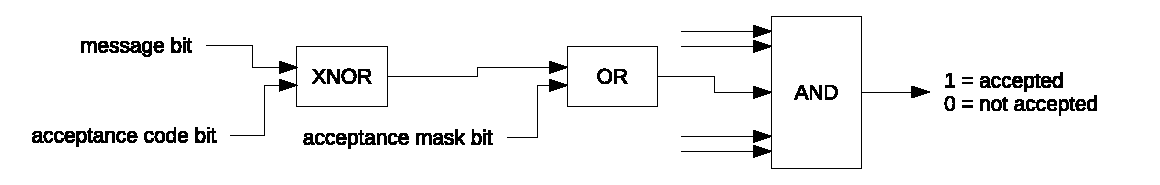
\includegraphics[width=0.8\textwidth]{./25-TWAI/figures/Acceptance_filter_en.eps}}
    \caption{Acceptance Filter}
    \label{Figure:Acceptance filter}
\end{figure}


\subsubsection{Single Filter Mode}

Single Filter Mode is enabled by setting the \hyperref[fielddesc:TWAIRXFILTERMODE]{TWAI\_RX\_FILTER\_MODE} bit to 1. This will cause the 32-bit code and mask values to define a single filter. The single filter can filter the following bits of a Data or Remote Frame:

\begin{itemize}
    \item SFF
    \begin{itemize}
        \item The entire 11-bit ID
        \item RTR bit
        \item Data byte 1 and Data byte 2
    \end{itemize}
    \item EFF
    \begin{itemize}
        \item The entire 29-bit ID
        \item RTR bit
    \end{itemize}
\end{itemize}

The following Figure \ref{Figure:Single Filter Mode} illustrates how the 32-bit code and mask values will be interpreted under Single Filter Mode.

\begin{figure}[ht]
    \centering
    \fbox{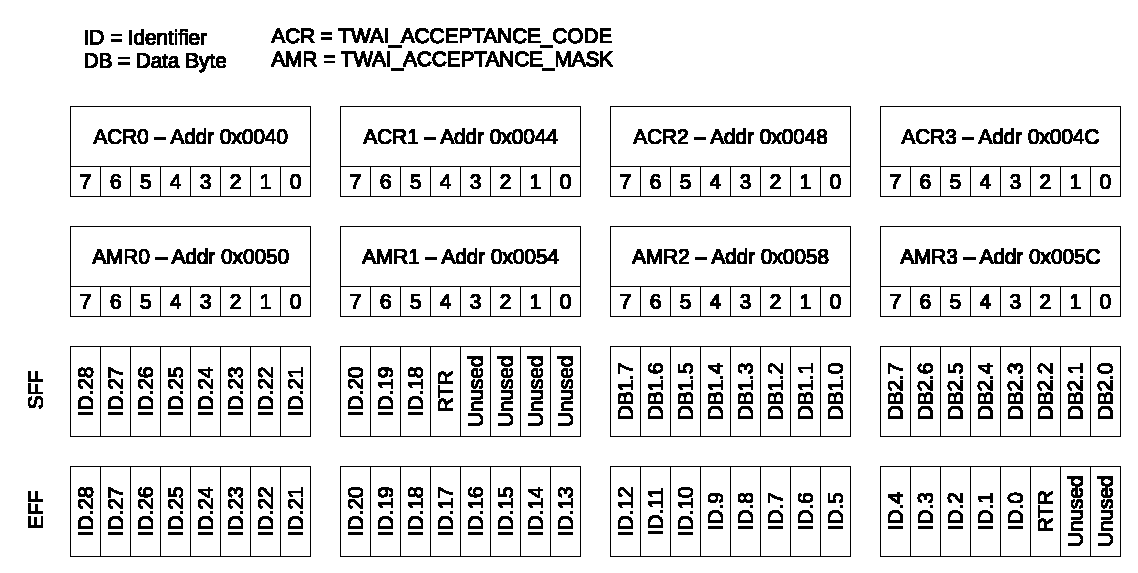
\includegraphics[width=0.8\textwidth]{./25-TWAI/figures/Single_Filter_Mode_en.eps}}
    \caption{Single Filter Mode}
    \label{Figure:Single Filter Mode}
\end{figure}

\subsubsection{Dual FIlter Mode}

Dual Filter Mode is enabled by setting the \hyperref[fielddesc:TWAIRXFILTERMODE]{TWAI\_RX\_FILTER\_MODE} bit to 0. This will cause the 32-bit code and mask values to define a two separate filters, referred to as filter 1 or two. Under Dual Filter Mode, a message will be accepted if it is accepted by one of the two filters.

The two filters can filter the following bits of a Data or Remote Frame:

\begin{itemize}
    \item SFF
    \begin{itemize}
        \item The entire 11-bit ID
        \item RTR bit
        \item Data byte 1 (for filter 1 only)
    \end{itemize}
    \item EFF
    \begin{itemize}
        \item The first 16 bits of the 29-bit ID
    \end{itemize}
\end{itemize}

The following Figure \ref{Figure:Dual Filter Mode} illustrates how the 32-bit code and mask values will be interpreted under Dual Filter Mode.

\begin{figure}[ht!]
    \centering
    \fbox{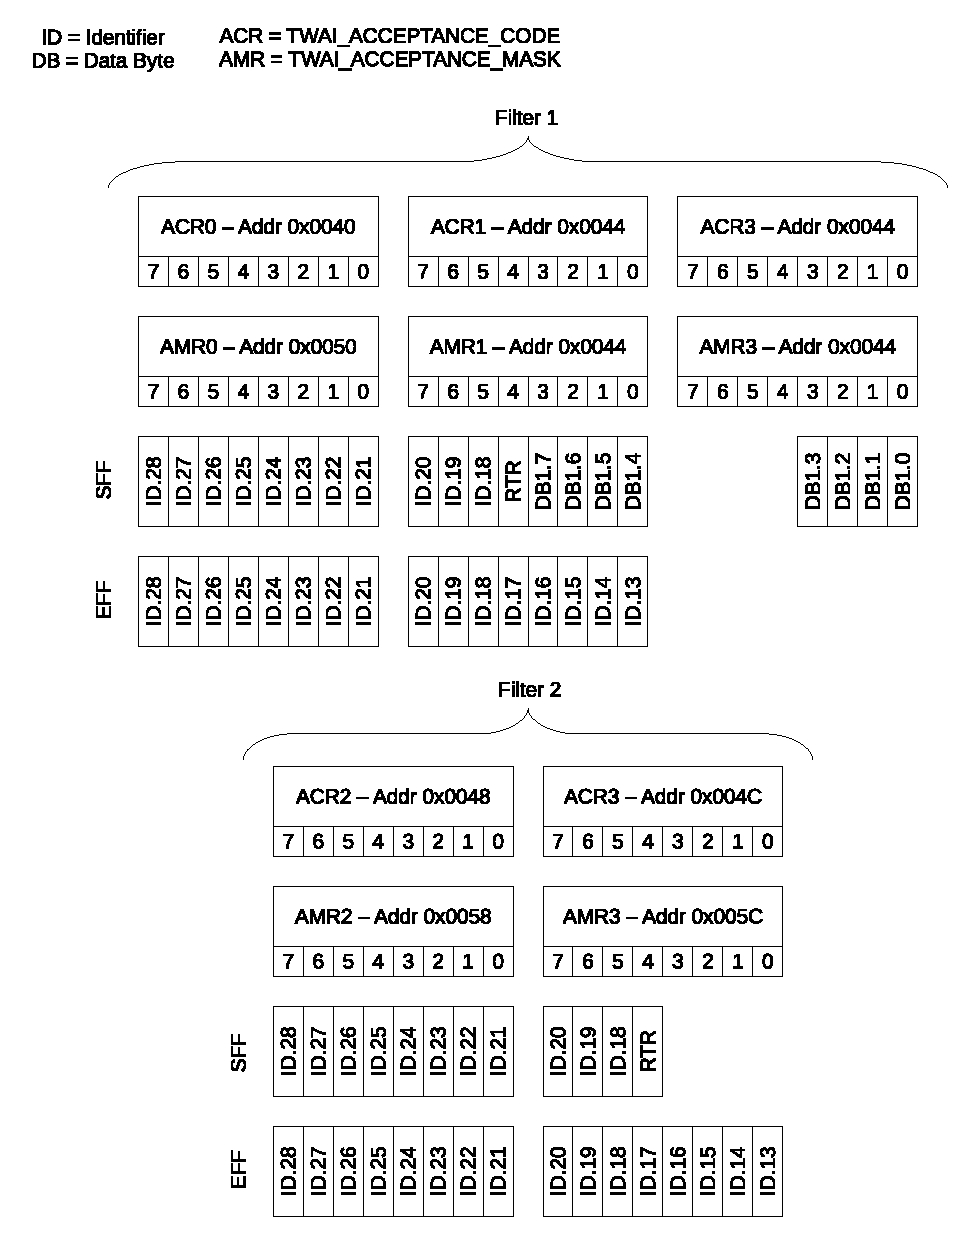
\includegraphics[width=0.8\textwidth]{./25-TWAI/figures/Dual_Filter_Mode_en.eps}}
    \caption{Dual Filter Mode}
    \label{Figure:Dual Filter Mode}
\end{figure}

\subsection{Error Management}

The TWAI protocol requires that each TWAI node maintains the Transmit Error Count (TEC) and Receive Error Count (REC). The value of both error counts determine the current error state of the TWAI controller (i.e., Error Active, Error Passive, Bus-Off). The TWAI controller stores the TEC and REC values in the \hyperref[regdesc:TWAITXERRCNTREG]{TWAI\_TX\_ERR\_CNT\_REG} and \hyperref[regdesc:TWAIRXERRCNTREG]{TWAI\_RX\_ERR\_CNT\_REG} respectively, and can be read by the CPU at anytime. In addition to the error states, the TWAI controller also offers an Error Warning Limit (EWL) feature that can warn the user regarding the occurrence of severe bus errors before the TWAI controller enters the Error Passive state.

The current error state of the TWAI controller is indicated via a combination of the following values and status bits: TEC, REC, \hyperref[fielddesc:TWAIERRST]{TWAI\_ERR\_ST}, and \hyperref[fielddesc:TWAIBUSOFFST]{TWAI\_BUS\_OFF\_ST}. Certain changes to these values and bits will also trigger interrupts, thus allowing the users to be notified of error state transitions (see section \ref{subsubsec:interrupt-management}). The following figure \ref{Figure:Error_State_Transtion} shows the relation between the error states, values and bits, and error state related interrupts.

\begin{figure}[ht!]
    \centering
    \fbox{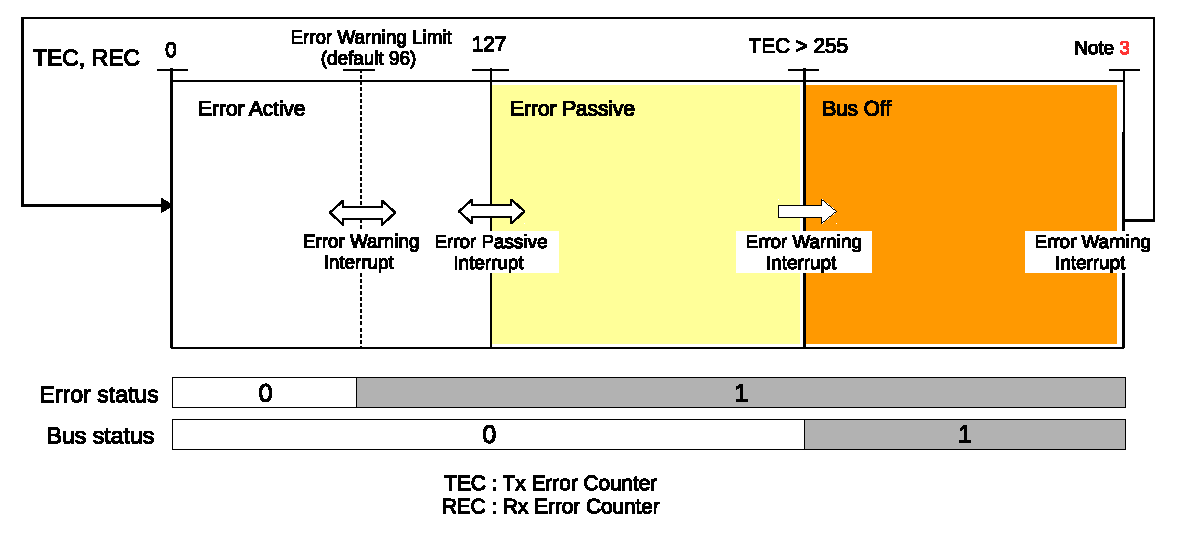
\includegraphics[width=0.8\textwidth]{./25-TWAI/figures/Error_State_Transition_20190625_en.eps}}
    \caption{Error State Transition}
    \label{Figure:Error_State_Transtion}
\end{figure}

\subsubsection{Error Warning Limit}

The Error Warning Limit (EWL) feature is a configurable threshold value for the TEC and REC, where if exceeded, will trigger an interrupt. The EWL is intended to serve as a warning about severe TWAI bus errors, and is triggered before the TWAI controller enters the Error Passive state. The EWL is configured in the \hyperref[regdesc:TWAIERRWARNINGLIMITREG]{TWAI\_ERR\_WARNING\_LIMIT\_REG} and can only be configured whilst the TWAI controller is in Reset Mode. The \hyperref[regdesc:TWAIERRWARNINGLIMITREG]{TWAI\_ERR\_WARNING\_LIMIT\_REG} has a default value of 96.
When the values of TEC and/or REC are larger than or equal to the EWL value, the \hyperref[fielddesc:TWAIERRST]{TWAI\_ERR\_ST} bit is immediately set to 1. Likewise, when the values of both the TEC and REC are smaller than the EWL value, the \hyperref[fielddesc:TWAIERRST]{TWAI\_ERR\_ST} bit is immediately reset to 0. The Error Warning Interrupt is triggered whenever the value of the \hyperref[fielddesc:TWAIERRST]{TWAI\_ERR\_ST} bit (or the \hyperref[fielddesc:TWAIBUSOFFST]{TWAI\_BUS\_OFF\_ST}) changes.


\subsubsection{Error Passive}

The TWAI controller is in the Error Passive state when the TEC or REC value exceeds 127. Likewise, when both the TEC and REC are less than or equal to 127, the TWAI controller enters the Error Active state. The Error Passive Interrupt is triggered whenever the TWAI controller transitions from the Error Active state to the Error Passive state or vice versa.

\subsubsection{Bus-Off and Bus-Off Recovery}

The TWAI controller enters the Bus-Off state when the TEC value exceeds 255. On entering the Bus-Off state, the TWAI controller will automatically do the following:

\begin{itemize}
    \item Set REC to 0
    \item Set TEC to 127
    \item Set the \hyperref[fielddesc:TWAIBUSOFFST]{TWAI\_BUS\_OFF\_ST} bit to 1
    \item Enter Reset Mode
\end{itemize}

The Error Warning Interrupt is triggered whenever the value of the \hyperref[fielddesc:TWAIBUSOFFST]{TWAI\_BUS\_OFF\_ST} bit (or the \hyperref[fielddesc:TWAIERRST]{TWAI\_ERR\_ST} bit) changes.

To return to the Error Active state, the TWAI controller must undergo Bus-Off recovery. Bus-Off recovery requires the TWAI controller to observe 128 occurrences of 11 consecutive Recessive bits on the bus. To initiate Bus-Off recovery (after entering the Bus-Off state), the TWAI controller should enter Operation Mode by setting the \hyperref[fielddesc:TWAIRESETMODE]{TWAI\_RESET\_MODE} bit to 0.
The TEC tracks the progress of Bus-Off recovery by decrementing the TEC each time the TWAI controller observes 11 consecutive Recessive bits. When Bus-Off recovery has completed (i.e., TEC has decremented from 127 to 0), the \hyperref[fielddesc:TWAIBUSOFFST]{TWAI\_BUS\_OFF\_ST} bit will automatically be reset to 0, thus triggering the Error Warning Interrupt.

\subsection{Error Code Capture}

The Error Code Capture (ECC) feature allows the TWAI controller to record the error type and bit position of a TWAI bus error in the form of an error code. Upon detecting a TWAI bus error, the Bus Error Interrupt is triggered and the error code is recorded in the \hyperref[regdesc:TWAIERRCODECAPREG]{TWAI\_ERR\_CODE\_CAP\_REG}. Subsequent bus errors will trigger the Bus Error Interrupt, but their error codes will not be recorded until the current error code is read from the \hyperref[regdesc:TWAIERRCODECAPREG]{TWAI\_ERR\_CODE\_CAP\_REG}.

The following Table \ref{table:ECC_REG1} shows the fields of the \hyperref[regdesc:TWAIERRCODECAPREG]{TWAI\_ERR\_CODE\_CAP\_REG}:

\begin{longtable}[c]{|p{1.4cm}|p{1.4cm}|p{1.4cm}|p{1.4cm}|p{1.4cm}|p{1.4cm}|p{1.4cm}|p{1.4cm}|p{1.4cm}|}
    \caption{Bit Information of \hyperref[regdesc:TWAIERRCODECAPREG]{TWAI\_ERR\_CODE\_CAP\_REG}; TWAI Address 0x30}
    \label{table:ECC_REG1}\\
    \hline
    \rowcolor{lightgray}
    Bit 31-8 & Bit 7 & Bit 6 & Bit 5 & Bit 4 & Bit 3 & Bit 2 & Bit 1 & Bit 0\\\hline
    Reserved & ERRC.1$^1$ & ERRC.0$^1$ & DIR$^2$ & SEG.4$^3$ & SEG.3$^3$ & SEG.2$^3$ & SEG.1$^3$ & SEG.0$^3$\\
    \hline
\end{longtable}
\vspace{-1.5em}
{\bfseries Notes:}\\
\begin{itemize}
    \item ERRC: The Error Code (ERRC) indicates the type of bus error: 00 for bit error, 01 for form error, 10 for stuff error, 11 for other type of error.
    \item DIR: The Direction (DIR) indicates whether the TWAI controller was transmitting or receiving when the bus error: 0 for Transmitter, 1 for Receiver.
    \item SEG: The Error Segment (SEG) indicates which segment of the TWAI message (i.e., bit position) the bus error occurred at.
\end{itemize}

The following Table \ref{table:Bit_information} shows how to interpret the SEG.0 to SEG.4 bits.

\begin{longtable}[c]{|p{2cm}<{\centering}|p{2cm}<{\centering}|p{2cm}<{\centering}|p{2cm}<{\centering}|p{2cm}<{\centering}|p{4cm}|}
    \caption{Bit Information of Bits SEG.4 - SEG.0}
    \label{table:Bit_information}\\
    \hline
    \rowcolor{lightgray}
   Bit SEG.4 & Bit SEG.3 & Bit SEG.2 & Bit SEG.1 & Bit SEG.0 & Description
   \\\hline
   \endfirsthead

   \hline
   \rowcolor{lightgray}
   Bit SEG.4 & Bit SEG.3 & Bit SEG.2 & Bit SEG.1 & Bit SEG.0 & Description
   \\\hline
   \endhead
   \endfoot
   \hline
   \endlastfoot

    0 & 0 & 0 & 1 & 1 & start of frame
    \\\hline
    0 & 0 & 0 & 1 & 0 & ID.28 to ID.21
    \\\hline
    0 & 0 & 1 & 1 & 0 & ID.20 to ID.18
    \\\hline
    0 & 0 & 1 & 0 & 0 & bit SRTR$^1$
    \\\hline
    0 & 0 & 1 & 0 & 1 & bit IDE$^2$
    \\\hline
    0 & 0 & 1 & 1 & 1 & ID.17 to ID.13
    \\\hline
    0 & 1 & 1 & 1 & 1 & ID.12 to ID.5
    \\\hline
    0 & 1 & 1 & 1 & 0 & ID.4 to ID.0
    \\\hline
    0 & 1 & 1 & 0 & 0 & bit RTR
    \\\hline
    0 & 1 & 1 & 0 & 1 & reserved bit 1
    \\\hline
    0 & 1 & 0 & 0 & 1 & reserved bit 0
    \\\hline
    0 & 1 & 0 & 1 & 1 & data length code
    \\\hline
    0 & 1 & 0 & 1 & 0 & data field
    \\\hline
    0 & 1 & 0 & 0 & 0 & CRC sequence
    \\\hline
    1 & 1 & 0 & 0 & 0 & CRC delimiter
    \\\hline
    1 & 1 & 0 & 0 & 1 & acknowledge slot
    \\\hline
    1 & 1 & 0 & 1 & 1 & acknowledge delimiter
    \\\hline
    1 & 1 & 0 & 1 & 0 & end of frame
    \\\hline
    1 & 0 & 0 & 1 & 0 & intermission
    \\\hline
    1 & 0 & 0 & 0 & 1 & active error flag
    \\\hline
    1 & 0 & 1 & 1 & 0 & passive error flag
    \\\hline
    1 & 0 & 0 & 1 & 1 & tolerate dominant bits
    \\\hline
    1 & 0 & 1 & 1 & 1 & error delimiter
    \\\hline
    1 & 1 & 1 & 0 & 0 & overload flag
    \\\hline
\end{longtable}
\vspace{-1.5em}
{\bfseries Notes:}\\
\begin{itemize}
    \item Bit RTR: under Standard Frame Format.
    \item Identifier Extension Bit: 0 for Standard Frame Format.
\end{itemize}

\subsection{Arbitration Lost Capture}

The Arbitration Lost Capture (ALC) feature allows the TWAI controller to record the bit position where it loses arbitration. When the TWAI controller loses arbitration, the bit position is recorded in the \hyperref[regdesc:TWAIARB LOST CAPREG]{TWAI\_ARB LOST CAP\_REG} and the Arbitration Lost Interrupt is triggered.

Subsequent loses in arbitration will trigger the Arbitration Lost Interrupt, but will not be recorded in the \hyperref[regdesc:TWAIARB LOST CAPREG]{TWAI\_ARB LOST CAP\_REG} until the current Arbitration Lost Capture is read from the \hyperref[regdesc:TWAIERRCODECAPREG]{TWAI\_ERR\_CODE\_CAP\_REG}.

Table \ref{table:ALC_REG} illustrates the bit fields of the \hyperref[regdesc:TWAIERRCODECAPREG]{TWAI\_ERR\_CODE\_CAP\_REG} whilst Figure \ref{Figure:TWAI_arbitration_lost_capture} illustrates the bit positions of a TWAI message.

\begin{longtable}[c]{|p{2.3cm}|p{2.3cm}|p{2.3cm}|p{2.3cm}|p{2.3cm}|p{2.3cm}|}
    \caption{Bit Information of \hyperref[regdesc:TWAIARB LOST CAPREG]{TWAI\_ARB LOST CAP\_REG}; TWAI Address 0x2c}
    \label{table:ALC_REG}
    \\\hline
    \rowcolor{lightgray}
  Bit 31-5 & Bit 4 & Bit 3 & Bit 2 & Bit 1 & Bit 0\\ \hline
   Reserved & BITNO.4$^1$ & BITNO.3$^1$ & BITNO.2$^1$ & BITNO.1$^1$ & BITNO.0$^1$\\\hline
\end{longtable}
\vspace{-1.5em}
{\bfseries Notes: }\\
\begin{itemize}
    \item BITNO: Bit Number (BITNO) indicates the nth bit of a TWAI message where arbitration was lost.
\end{itemize}

\begin{figure}[ht!]
    \centering
    \fbox{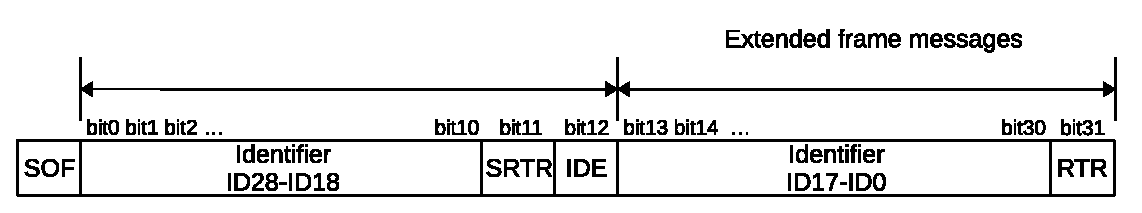
\includegraphics[width=0.9\textwidth]{./25-TWAI/figures/Positions_of_Arbitration_Lost_Bits_20190625_en.eps}}
    \caption{Positions of Arbitration Lost Bits}
    \label{Figure:TWAI_arbitration_lost_capture}
\end{figure}

\hypertarget{twai-reg-summ}{}
\section{Register Summary}
\label{chapter:Register_Summary}

The addresses in this section are relative to the TWAI base address provided in Table \ref{table:Peripheral_Address_Mapping} in Chapter \ref{mod:sysmem} \textit{\nameref{mod:sysmem}}.

The abbreviations given in Column \textbf{Access} are explained in Section \hyperref[glossary-access-types]{\textit{Access Types for Registers}}.


\subfile{\modulefiles/twai-reg-summ_en}

\section{Registers}
\label{chapter:Register_Description}

The addresses in this section are relative to the TWAI base address provided in Table \ref{table:Peripheral_Address_Mapping} in Chapter \ref{mod:sysmem} \textit{\nameref{mod:sysmem}}. The absolute register addresses are listed in Section \ref{chapter:Register_Summary} \textit{\nameref{chapter:Register_Summary}}. 

For how to program reserved fields, please refer to Section \hyperref[programming-reserved-field]{\textit{Programming Reserved Register Field}}.

\subfile{\modulefiles/twai-reg_en}

\end{document}
